\lstinputlisting[language=bash,basicstyle=\small]{python_codes/fieldstone_54/keywords.ascii}

\begin{center}
Code at \url{https://github.com/cedrict/fieldstone/tree/master/python_codes/fieldstone_54}
\end{center}

\par\noindent\rule{\textwidth}{0.4pt}



This stone implements three different free surface/mesh deformation algorithms. 
The first one has all the nodes move with the computed velocity (Lagrangian method)
and is coined 'method 1'. 
The second one ('method 2') only has the top row of nodes moving with the computed velocity, 
while all the nodes underneath are static (this is obviously not a viable method for 
large deformations). 
The third one ('method 3') is the method used in ASPECT and described in Rose et al (2017) \cite{robh17}.
Its implementation is described in Section~\ref{sec:freesurface}.

%...........................................................
\subsubsection*{Experiment 1 - relaxation of topography}

The domain is a 2D Cartesian box of size 512$\times$512km, with free slip on left, 
bottom and right sides, free surface at the top. 
Mantle material characterised by $\rho_m=3200$ and $\eta_m=10^{22}$. 
Gravity is vertical and Earth like. 
The surface is perturbed at startup by $\delta y = A \cos (\pi x /L_x)$ with $A$=1km.
200 time steps with $\delta t=10$kyr are carried out.
The root mean square velocity, the total volume of the domain, the min/max elevation
values of the surface are recorded over time. 

\begin{center}
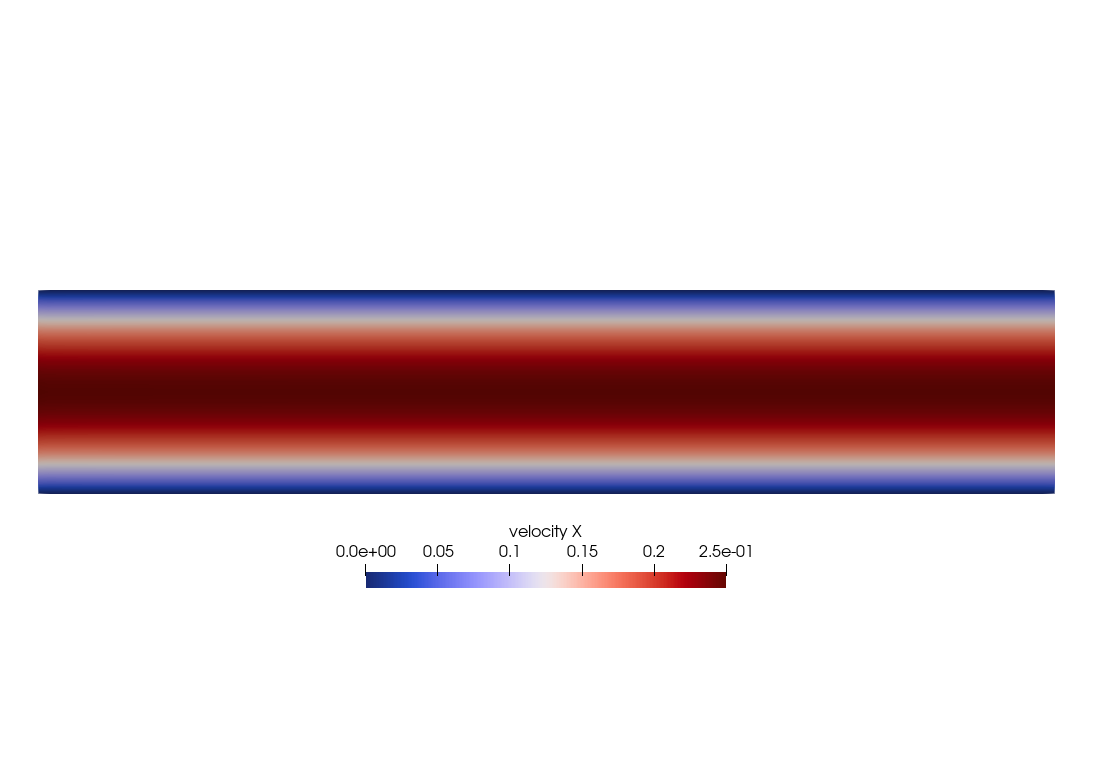
\includegraphics[width=7.5cm]{python_codes/fieldstone_54/images/exp1/u}
\includegraphics[width=7.5cm]{python_codes/fieldstone_54/images/exp1/v}\\
{\captionfont velocity field at $t=0$ with resolution 24x24}
\end{center}

The results hereunder are obtained for all three methods at two different resolutions (16x16 
and 24x24 elements).
The plots on the left column are obtained with the movement of the top nodes being constrained in 
the vertical direction, while the plots on the right column are obtained with nodes being 
allowed to move in both $x$ and $y$ directions (note that for method 3 the normals are not -yet-
computed with the method of Eq. 49 in \cite{robh17} but instead by a simple geometric rule).

\begin{center}
a) \includegraphics[width=7cm]{python_codes/fieldstone_54/images/exp1/elevation_vert.pdf}
   \includegraphics[width=7cm]{python_codes/fieldstone_54/images/exp1/elevation_full.pdf}\\
b) \includegraphics[width=7cm]{python_codes/fieldstone_54/images/exp1/elevation_log_vert.pdf}
   \includegraphics[width=7cm]{python_codes/fieldstone_54/images/exp1/elevation_log_full.pdf}\\
c) \includegraphics[width=7cm]{python_codes/fieldstone_54/images/exp1/volume_vert.pdf}
   \includegraphics[width=7cm]{python_codes/fieldstone_54/images/exp1/volume_full.pdf}\\
d) \includegraphics[width=7cm]{python_codes/fieldstone_54/images/exp1/vrms_vert.pdf}
   \includegraphics[width=7cm]{python_codes/fieldstone_54/images/exp1/vrms_full.pdf}\\
e) \includegraphics[width=7cm]{python_codes/fieldstone_54/images/exp1/surface_topography_200_vert.pdf}
   \includegraphics[width=7cm]{python_codes/fieldstone_54/images/exp1/surface_topography_200_full.pdf}\\
{\captionfont 
a) min/max of free surface topo as a function of time; 
b) free surface topo maximum (in log scale) as a function of time; 
c) measured volume of the domain with numerical quadrature normalised by the expected volume $L_xL_y$;
d) root mean square velocity as a function of time;
e) final elevation at the 200th time step.}
\end{center}

%...........................................................
\subsubsection*{Experiment 2,3 - extension}

We now consider a rectangular domain (crust sized) of $128\times32$km, discretised by means of $40\times10$ elements.
The fluid is identical to the one above and so is gravity. 
Extensional boundary conditions are applied. In the first case, a 1cm/yr horizontal velocity is applied on both sides, while in the second case a 2cm/yr velocity is applied on the right while 0 is prescribed to the left. Free slip conditions are otherwise prescribed on the sides and bottom. 100 time steps are carried out with $\delta t=10^4$yr. Only method 3 is used here.

\begin{center}
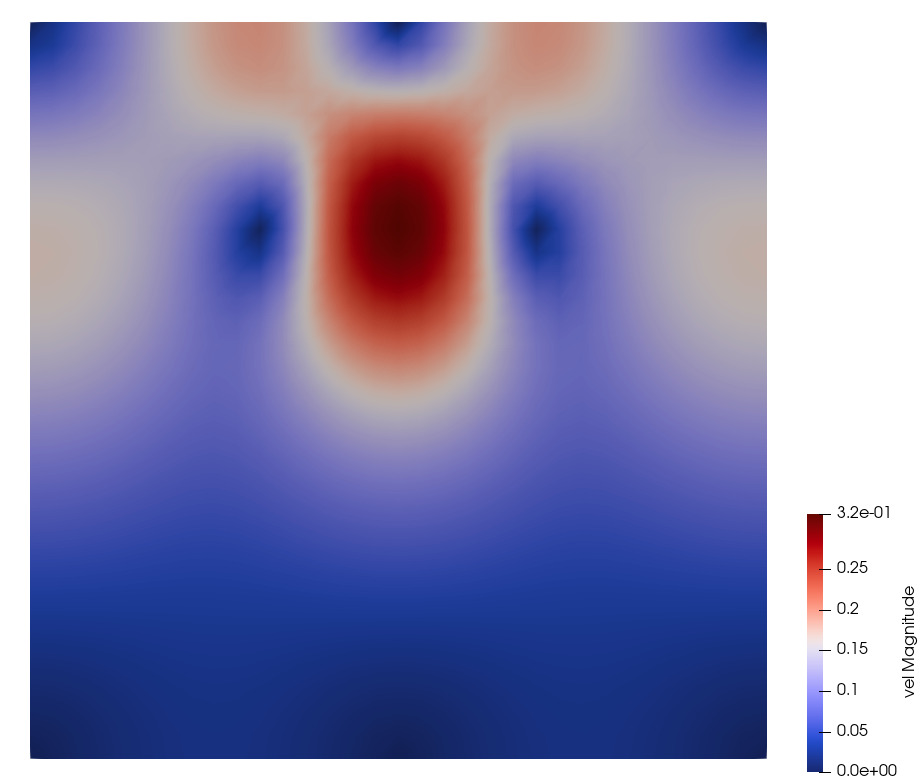
\includegraphics[width=13cm]{python_codes/fieldstone_54/images/exp2-3/vel0}\\
{\captionfont Velocity field for both experiments at $t=0$.}
\end{center}


Despite the asymmetry in the boundary conditions, we expect the same evolution of the domain geometry. This is indeed what we recover with surprising accuracy. 'vert' stands for only vertical movement allowed (i.e. $n_x=0$, 
$n_y=1$) while 'both dir' stands for the use of dynamically computed normal vectors (based on geometrical consideration).

\begin{center}
\includegraphics[width=7cm]{python_codes/fieldstone_54/images/exp2-3/volume.pdf}
\includegraphics[width=7cm]{python_codes/fieldstone_54/images/exp2-3/surface.pdf}\\
{\captionfont Left: time evolution of the normalised volume for both boundary condition types; Right: surface at the end of the simulation.}
\end{center}


\begin{center}
\includegraphics[width=7cm]{python_codes/fieldstone_54/images/exp2-3/vrms.pdf}
\includegraphics[width=7cm]{python_codes/fieldstone_54/images/exp2-3/elevation.pdf}\\
{\captionfont Left: Root mean square velocity as a function of time; Right: time evolution of the elevation (min and max virtually indistinguishable).} 
\end{center}


%...........................................................
\subsubsection*{Experiment 4,5 - extension with bottom inflow}

This is the same setup as above, but we now impose an influx boundary condition at the bottom: $v=0.5cm$ (this balances the outflux exactly) and 
the horizontal component at the bottom is set to the left value (-1 or 0 cm/yr) for $x\leq L_x/2$ and to the right value +1 or +2 cm/yr for $x\geq L_x/2$.

\begin{center}
\includegraphics[width=7cm]{python_codes/fieldstone_54/images/exp4-5/volume.pdf}
\includegraphics[width=7cm]{python_codes/fieldstone_54/images/exp4-5/surface.pdf}\\
\includegraphics[width=7cm]{python_codes/fieldstone_54/images/exp4-5/vrms.pdf}
\includegraphics[width=7cm]{python_codes/fieldstone_54/images/exp4-5/elevation.pdf}\\
\end{center}

We can conclude that the 'vertical movement only' conserves volume/mass better and the free surface remains symmetrical unless the full normal is used which is simply explained by having $\vec{v}\cdot\vec{n}$ as a boundary condition: in the asymmetric extension case, the velocity is always to the right while the normal has an $x$ component which is negative and positive, therefore introducing an asymmetry in the surface boundary conditions.

\begin{center}
\includegraphics[width=9cm]{python_codes/fieldstone_54/images/exp4-5/v}\\
{\captionfont Top to bottom: 
symmetric extension, full normal vector; 
symmetric extension, vertical normal vector; 
asymmetric extension, full normal vector; 
asymmetric extension, vertical normal vector}
\end{center}

%...........................................................
\subsubsection*{Experiment 6 - pure advection test}

\begin{center}
\includegraphics[width=7cm]{python_codes/fieldstone_54/images/exp6/velp}\\
\includegraphics[width=7cm]{python_codes/fieldstone_54/images/exp6/surface.pdf}
\includegraphics[width=7cm]{python_codes/fieldstone_54/images/exp6/elevation.pdf}\\
{\captionfont Results after 100 time steps = 1Myr}
\end{center}

%...........................................................
\subsubsection*{Experiment 7 - pure advection test of a cosine bump}

The initial topography bump is given by
\[
y(x)=A \left[ 1+ \cos \left( \frac{x-x_0}{w} \pi \right) \right]
\]
with $A=1000$m, $x_0=0.345678L_x$ and $w=$15km. This is a somewhat ideal case 
since the transition from flat to bump is very smooth.

The viscosity is set to $10^{26}$Pa$\cdot$s so that the velocity of the 
viscous relaxation of the topography is negligible with regards to the advection velocity
(+1cm/yr on left and right boundaries). I also choose a resolution of 80x20 elements.

\begin{center}
\includegraphics[width=8cm]{python_codes/fieldstone_54/images/exp7/v}
\end{center}

If only the vertical normal is used then {\sl nothing} moves since the 
velocity is always perpendicular to the normal. 

What follows is obtained when the full normal is used. 
After 20 timesteps the topography has been advected and we already observe some 
visible asymmetry (and oscillations) on the surface:
\begin{center}
\includegraphics[width=11cm]{python_codes/fieldstone_54/images/exp7/surface.pdf}
\end{center}

On the following plots the left column shows $(\vec{\upnu}\cdot \vec{n})n_x$ 
as a function of the $x$-coordinate and the 
right column shows $(\vec{\upnu}\cdot \vec{n})n_y$, both for timesteps 1,2,3,5,10,20. 
Both quantities form the 
boundary conditions for the mesh deformation.  
Since I have chosen $x_0$ such that it does not fall on a node, the initial 
topography is {\sl not} symmetric and therefore the normal vectors at the nodes 
on the left and right of the peak are not identical. From the second timestep (the first one 
for which the free surface algo uses a non zero Stokes velocity as boundary condition)
we see that both components $(\vec{\upnu}\cdot \vec{n})n_x$ and $(\vec{\upnu}\cdot \vec{n})n_y$ are asymmetric! 


\begin{center}
\includegraphics[width=6cm]{python_codes/fieldstone_54/images/exp7/n_dov_v_nx_001.pdf}
\includegraphics[width=6cm]{python_codes/fieldstone_54/images/exp7/n_dov_v_ny_001.pdf}\\
\includegraphics[width=6cm]{python_codes/fieldstone_54/images/exp7/n_dov_v_nx_002.pdf}
\includegraphics[width=6cm]{python_codes/fieldstone_54/images/exp7/n_dov_v_ny_002.pdf}\\
\includegraphics[width=6cm]{python_codes/fieldstone_54/images/exp7/n_dov_v_nx_003.pdf}
\includegraphics[width=6cm]{python_codes/fieldstone_54/images/exp7/n_dov_v_ny_003.pdf}\\
\includegraphics[width=6cm]{python_codes/fieldstone_54/images/exp7/n_dov_v_nx_005.pdf}
\includegraphics[width=6cm]{python_codes/fieldstone_54/images/exp7/n_dov_v_ny_005.pdf}\\
\includegraphics[width=6cm]{python_codes/fieldstone_54/images/exp7/n_dov_v_nx_010.pdf}
\includegraphics[width=6cm]{python_codes/fieldstone_54/images/exp7/n_dov_v_ny_010.pdf}\\
\includegraphics[width=6cm]{python_codes/fieldstone_54/images/exp7/n_dov_v_nx_020.pdf}
\includegraphics[width=6cm]{python_codes/fieldstone_54/images/exp7/n_dov_v_ny_020.pdf}
\end{center}

The inescapable conclusion is that the algorithm (as it is now implemented with the normal 
vector) is incapable of advecting a bump. 

In what follows, the Stokes system is solved once, and the obtained velocity
is used to compute the mesh velocity boundary condition for the Laplace system. 
The resolution is set to 100x25. I have implemented the $L_2$ projection approach 
of \cite{robh17} for both Q1 and Q2 elements. For such a smooth topography the 
Q1 and geometrical approach (i.e. using geometrically computed normal vectors) are
very similar although Q1 produces tiny undershoots. Q2 however generates oscillations
which makes the computed velocity not suited as a boundary condition to move surface nodes. 

From left to right: horizontal component, vertical component, and vector form 
of the computed mesh velocity bc.

\begin{center}
\includegraphics[width=7cm]{python_codes/fieldstone_54/images/exp7/100x25/umesh}
\includegraphics[width=7cm]{python_codes/fieldstone_54/images/exp7/100x25/vmesh}\\
\includegraphics[width=11cm]{python_codes/fieldstone_54/images/exp7/100x25/velmesh}
\end{center}

I haven't used any of the projections to carry out timestepping.

%......................................................................
\subsubsection*{Experiment 8 - pure advection test of a pyramidal bump}

This is a nearly identical experiment as the previous one, but now the bump is 
composed of two straight lines, of slopes $\pm 0.1$.
Pyramid centered at $x=0.345678L_x$, of half width 15km. $\rho=3000$, $\eta=10^{26}$.
Resolution 60x15. +1cm/yr prescribed on left and right. dt=10kyr. 

\begin{center}
\includegraphics[width=9cm]{python_codes/fieldstone_54/images/exp8/v}
\end{center}

\begin{center}
\includegraphics[width=8cm]{python_codes/fieldstone_54/images/exp8/surface.pdf}\\
\includegraphics[width=10cm]{python_codes/fieldstone_54/images/exp8/bc_vmesh.pdf}
\end{center}

Results are not crazy bad, but we should be able to do better ... the pyramid 
becomes more and more deformed after only 20km of advection (but surprisingly retains its height). 



In what follows, the Stokes system is solved once, and the obtained velocity
is used to compute the mesh velocity boundary condition for the Laplace system. 
The resolution is set to 100x25. I have implemented the $L_2$ projection approach 
of \cite{robh17} for both Q1 and Q2 elements. For such a broken line topography the 
geometrical approach (i.e. using geometrically computed normal vectors) is better.
Q1 and Q2 both produce under/overshoots/oscillations with no clear winner. 

From left to right: horizontal component, vertical component, and vector form 
of the computed mesh velocity bc.

\begin{center}
\includegraphics[width=7cm]{python_codes/fieldstone_54/images/exp8/100x25/umesh}
\includegraphics[width=7cm]{python_codes/fieldstone_54/images/exp8/100x25/vmesh}\\
\includegraphics[width=11cm]{python_codes/fieldstone_54/images/exp8/100x25/velmesh}
\end{center}

I haven't used any of the projections to carry out timestepping.

%......................................................................


%......................................................................
\subsubsection*{Experiment 9 - Rayleigh-Taylor instability}


The setup originates in Kaus et al (2010) \cite{kamm10}.
It is a Rayleigh-Taylor instability of a dense, more viscous 
layer ($\rho=3300kg/m^3$ , $\eta=10^{21}Pa\cdot s$), 
sinking through a less dense fluid ($\rho=3200 kg/m^3$ , $\eta=10^{20}Pa\cdot s$). 
Side boundaries are free slip, the lower boundary is no-slip and the upper boundary 
is a free surface. 
The box is 500 x 500 km in size, and gravitational acceleration was 9.81m/s$^2$ . 
The initial perturbation was sinusoidal with initial amplitude $A$ of 5 km (i.e. 1\%
of the box size) and centered at $y_0=400$km:
\[
y(x)=y_0 - A \cos(2\pi x/L_x)
\]
The position $y(t)$ of the free surface point situated at $x=L_x$ 
is monitored and plotted ...

\begin{center}
\includegraphics[width=5cm]{python_codes/fieldstone_54/images/exp9/robh17}\\
{\captionfont Taken from Rose et al (2017) \cite{robh17}.}
\end{center}

Because I do not have compositional fields or markers implemented in this code I have 
to align the mesh with the initial sinusoidal perturbation and run the model in 
Lagrangian mode. Also, as shown in \cite{kamm10}, this experiment is prone to drunken sailor 
instabilities and I have therefore fixed dt=2500yr with a 25x25 resolution.
As a consequence, the model will run until elements become too distorted. 

\begin{center}
\includegraphics[width=13cm]{python_codes/fieldstone_54/images/exp9/kamm10}\\
{\captionfont Taken from Kaus et al (2010) \cite{kamm10}.}
\end{center}
Kaus et al show that the system is stable for $\delta t=2500$yr and 
quickly unstable for $\delta t=5000$yr. This is also what we observe:

\begin{center}
\includegraphics[width=7cm]{python_codes/fieldstone_54/images/exp9/volume.pdf}
\includegraphics[width=7cm]{python_codes/fieldstone_54/images/exp9/elev.pdf}\\
{\captionfont Results obtained with method=1. 25x25 resolution.}
\end{center}

\begin{center}
\includegraphics[width=5cm]{python_codes/fieldstone_54/images/exp9/rho0000}
\includegraphics[width=5cm]{python_codes/fieldstone_54/images/exp9/rho0040}
\includegraphics[width=5cm]{python_codes/fieldstone_54/images/exp9/rho0050}\\
\includegraphics[width=5cm]{python_codes/fieldstone_54/images/exp9/rho0051}
\includegraphics[width=5cm]{python_codes/fieldstone_54/images/exp9/rho0052}
\includegraphics[width=5cm]{python_codes/fieldstone_54/images/exp9/rho0053}\\
{\captionfont mesh at time steps 0,40,50,51,52,53 for $\delta t=5000$yr.}
\end{center}






